\documentclass{article}

% Chinese Support using xeCJK
% \usepackage{xeCJK}
% \setCJKmainfont{SimSun}

% Chinese Support using CTeX
\usepackage{ctex}

% Math Support
\usepackage{amsmath}
\usepackage{amsfonts}
\usepackage{amssymb}
\usepackage{wasysym}

% Graphics Support
\usepackage{graphicx}
\usepackage{float}

% Reduced page margin
\usepackage{geometry}
\geometry{a4paper,scale=0.8}

\usepackage{caption}
\usepackage{subcaption}

% d and e should be math operators
\newcommand*{\dif}{\mathop{}\!\mathrm{d}}
\newcommand*{\md}{\mathop{}\!\mathrm{d}}
\newcommand*{\me}{\mathrm{e}}

% No indent for each paragraph
\usepackage{parskip}
\setlength{\parindent}{0cm}

% Bold style for Greek letters
\usepackage{bm}
\let\Oldmathbf\mathbf
\renewcommand{\mathbf}[1]{\boldsymbol{\Oldmathbf{#1}}}

% More space for dfrac in cell
\usepackage{cellspace}
\setlength{\cellspacetoplimit}{5pt}
\setlength{\cellspacebottomlimit}{5pt}

% SI units
%\usepackage{siunitx}
%\let\Oldsi\si
%\renewcommand{\si}[1]{\  \Oldsi{#1}}
\newcommand{\si}[1]{\  \mathrm{#1}}

\usepackage{fancyhdr}
\pagestyle{fancy}
\fancyhf{}
\lhead{本文档TeX源代码地址:https://github.com/hxp-plus/Notes/tree/master/Qumntum-Mechenics/Summary}
\rfoot{第 \thepage 页}
\renewcommand{\headrulewidth}{1pt}
\renewcommand{\footrulewidth}{1pt}

\usepackage{authblk}
\title{量子力学学习笔记}
\author{胡喜平}
\affil{https://hxp.plus/}
\date{1970年1月1日}

\begin{document}
\maketitle\thispagestyle{fancy}

\section{数学基础}

\subsection{三位旋转坐标系}

下图中$x'$和$x$、$y$、$z$的夹角为$\alpha_1$、$\beta_1$、$\gamma_1$,$y'$和$x$、$y$、$z$的夹角为$\alpha_2$、$\beta_2$、$\gamma_2$,$z'$和$x$、$y$、$z$的夹角为$\alpha_3$、$\beta_3$、$\gamma_3$

\begin{figure}[H]
  \centering
  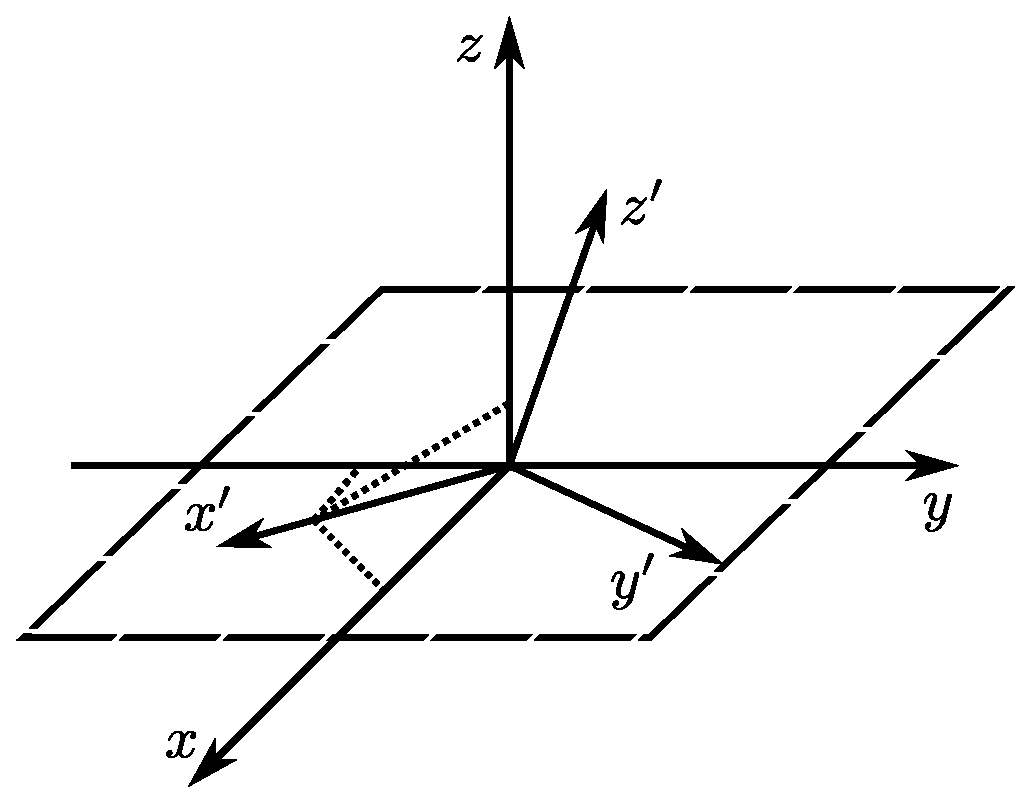
\includegraphics[width=0.5\linewidth]{figures/三维旋转坐标系}
  \caption{三维旋转坐标系}
  \label{fig:三维旋转坐标系}
\end{figure}

以$x$方向为例

\begin{equation*}
  \begin{aligned}
    x' = x \cos \alpha_1 + y \cos \beta_1 + z \cos \gamma_1
  \end{aligned}
\end{equation*}

$y$、$z$同理

\begin{equation*}
  \begin{aligned}
    y' &= y \cos \alpha_2 + y \cos \beta_2 + z \cos \gamma_2 \\
    z' &= x \cos \alpha_3 + y \cos \beta_3 + z \cos \gamma_3
  \end{aligned}
\end{equation*}

因此旋转矩阵为

\begin{equation*}
  R = 
  \begin{aligned}
    \left[
      \begin{array}{ccc}
       \cos \alpha_{1} & \cos \beta_{1} & \cos \gamma_{1}\\
       \cos \alpha_{2} & \cos \beta_{2} & \cos \gamma_{2}\\
       \cos \alpha_{3} & \cos \beta_{3} & \cos \gamma_{3}
      \end{array}
    \right ]
  \end{aligned}
\end{equation*}

则

\begin{equation*}
  \begin{aligned}
    \left[
      \begin{array}{ccc}
        x'\\
        y'\\
        z' 
      \end{array}
    \right ]
  \end{aligned}
  = R
  \begin{aligned}
    \left[
      \begin{array}{ccc}
        x\\
        y\\
        z 
      \end{array}
    \right ]
  \end{aligned}
  = 
  \begin{aligned}
    \left[
      \begin{array}{ccc}
       \cos \alpha_{1} & \cos \beta_{1} & \cos \gamma_{1}\\
       \cos \alpha_{2} & \cos \beta_{2} & \cos \gamma_{2}\\
       \cos \alpha_{3} & \cos \beta_{3} & \cos \gamma_{3}
      \end{array}
    \right ]
  \end{aligned}
  \begin{aligned}
    \left[
      \begin{array}{ccc}
        x\\
        y\\
        z 
      \end{array}
    \right ]
  \end{aligned}
\end{equation*}

\subsection{矢量分析}

Kronecker符号定义为:

\begin{equation*}
  \begin{aligned}
    \delta_{ij} =
  \end{aligned}
  \left\{
  \begin{aligned}
    & 1 && i=j \\
    & 0 && i\neq j
  \end{aligned}
  \right.
\end{equation*}

基矢之间的点乘可以表示为

\begin{equation*}
  \begin{aligned}
    \vec{e}_i \cdot \vec{e}_j = \delta_{ij}
  \end{aligned}
\end{equation*}

Levi-Civita张量定义为

\begin{equation*}
  \begin{aligned}
    \epsilon_{ijk} = 
  \end{aligned}
  \left\{
  \begin{aligned}
    & 1 && i,j,k=(1,2,3), (2,3,1),(3,1,2) \\
    & -1 && i,j,k=(3,2,1),(2,1,3),(1,3,2) \\
    & 0 && i=j\ \text{or}\ j = k \ \text{or}\ i=k
  \end{aligned}
  \right.
\end{equation*}

基矢之间的点乘可以表示为

\begin{equation*}
  \begin{aligned}
    \vec{e}_i \times \vec{e}_j = \epsilon_{ijk} \vec{e}_k
  \end{aligned}
\end{equation*}

其中运用了爱因斯坦求和转换,要对重复的字母$k$进行递归求和。

Levi-Civita张量还可以表示为

\begin{equation*}
  \begin{aligned}
    \epsilon_{ijk} = 
  \end{aligned}
  \begin{aligned}
    \left[
      \begin{array}{ccc}
       \delta_{i1} & \delta_{i2} & \delta_{i3}\\
       \delta_{j1} & \delta_{j2} & \delta_{j3}\\
       \delta_{k1} & \delta_{k2} & \delta_{k3}
      \end{array}
    \right ]
  \end{aligned}
\end{equation*}

矢量的点乘和叉乘可以表示为

\begin{equation*}
  \begin{aligned}
    & \vec{A} \cdot \vec{B} = \delta_{ij} A_i B_j = A_iB_i \\
    & \left( \vec{A} \times \vec{B} \right)_i = \epsilon_{ijk} A_j B_k
  \end{aligned}
\end{equation*}

常用的一些公式有

\begin{equation*}
  \begin{aligned}
    & \delta_{ij} \delta_{mj} = \delta_{i1} \delta_{m1} + \delta_{i2} \delta_{m2} + \delta_{i3} \delta_{m3} = \delta_{im} \\
    & \delta_{ii} = \delta_{11} + \delta_{22} + \delta_{33} = 3 \\
    & \epsilon_{ijk} \epsilon_{mnk} = \delta_{im} \delta_{jn} - \delta_{in} \delta_{jm}
  \end{aligned}
\end{equation*}

推论有

\begin{equation*}
  \begin{aligned}
    & \epsilon_{ijk} \epsilon_{mjk} = 2 \delta_{im} \\
    & \epsilon_{ijk} \epsilon_{ijk} = 6
  \end{aligned}
\end{equation*}

从此矢量的运算可以表示为

\begin{equation*}
  \begin{aligned}
    & \vec{A} + \vec{B} = \left( A_i + B_i \right) \vec{e}_i \\
    & \vec{A} \cdot \vec{B} = \left( A_i \vec{e}_i \right) \cdot \left( B_j \vec{e}_j \right) = \left( A_i B_j \right) \left( \vec{e}_i \cdot \vec{e}_j \right) = \delta_{ij} A_i B_j = A_i B_i \\
    & \vec{A} \times \vec{B} = \left( A_i \vec{e}_i \right) \times \left( B_j \vec{e}_j \right) = A_i B_j \left( \vec{e}_i \times \vec{e}_j \right) = \epsilon_{ijk} A_i B_j \vec{e}_k
  \end{aligned}
\end{equation*}

显然

\begin{equation*}
  \begin{aligned}
    \vec{A} \cdot \left( \vec{B} \times \vec{C} \right) &= \vec{A} \cdot \left( \epsilon_{ijk} B_i C_j \right) \vec{e}_k = \left( A_l \vec{e}_l \right) \left( \epsilon_{ijk} B_i C_j \vec{e}_k \right) = \delta_{lk} \epsilon_{ijk} A_l B_i C_j \\
    &= \epsilon_{ijk} A_k B_i C_j
  \end{aligned}
\end{equation*}


\begin{equation*}
  \begin{aligned}
    \vec{A} \times \left( \vec{B} \times \vec{C} \right) &= \vec{A} \times \left( \epsilon_{ijk} B_i C_j \vec{e}_k \right) = \epsilon_{mnl} A_m \left( \epsilon_{ijk} B_i C_j \vec{e}_k  \right)_n \vec{e}_l = \epsilon_{mnl} A_m \left( \epsilon_{ijn} B_i C_j \right) \vec{e}_l \\
    &= \epsilon_{mnl} \epsilon_{ijn} A_m B_i C_j \vec{e}_l = \left( \epsilon_{lmn} \epsilon_{ijn} \right) A_m B_i C_j \vec{e}_l \\
    &= \left( \delta_{li} \delta_{mj} - \delta_{lj} \delta_{mi} \right) A_m B_i C_j \vec{e}_l \\
    &= \left( A_m B_l C_m - A_m B_m C_l \right) \vec{e}_i = \left( A_m C_m \right) B_l \vec{e}_l - \left( A_m B_m \right) C_l \vec{e}_l \\
    &= \left( \vec{A} \cdot \vec{C} \right) \vec{B} - \left( \vec{A} \cdot \vec{B} \right) \vec{C}
  \end{aligned}
\end{equation*}

梯度算符可以简化为

\begin{equation*}
  \begin{aligned}
    \nabla = \vec{e}_1 \dfrac{\partial}{\partial x_1} +  \vec{e}_2 \dfrac{\partial}{\partial x_2} + \vec{e}_3 \dfrac{\partial}{\partial x_3} = \vec{e}_i \dfrac{\partial}{\partial x_i} = \vec{e}_i \partial_i 
  \end{aligned}
\end{equation*}

在直角坐标系中

\begin{equation*}
  \begin{aligned}
    \partial_i x_j = \dfrac{\partial x_j}{\partial x_i} = \delta_{ij} =  
  \end{aligned}
  \left\{
  \begin{aligned}
    & 1 && i=j \\
    & 0 && i \neq j
  \end{aligned}
  \right.
\end{equation*}

矢量的散度为

\begin{equation*}
  \begin{aligned}
    \nabla \cdot \vec{A} &= \vec{e}_i \partial_i \cdot \left( A_j \vec{e}_j \right) = \left( \vec{e}_i \cdot \vec{e}_j \right) \partial_i A_j + A_j \vec{e}_i \left( \partial_i \vec{e}_j \right) = \delta_{ij} \partial_i A_j = \partial_i A_i \\
    &= \partial_1 A_1 + \partial_2 A_2 + \partial_3 A_3 \\
    &= \dfrac{\partial A_1}{\partial x_1} + \dfrac{\partial A_2}{\partial x_2} + \dfrac{\partial A_3}{\partial x_3}   
  \end{aligned}
\end{equation*}

矢量场的旋度为

\begin{equation*}
  \begin{aligned}
    \nabla \times \vec{A} &= \left( \vec{e}_i \partial_i \right) \times \left( A_j \vec{e}_j \right) = \epsilon_{lmn} \left( \vec{e}_i \partial_i \right)_l \left( A_j \vec{e}_j \right)_m \vec{e}_n = \epsilon_{lmn} \partial_l A_m \vec{e}_n \\
    &= \left( \partial_2 A_3 - \partial_3 A_2 \right) \vec{e}_1 + \left( \partial_3 A_1 - \partial_1 A_3 \right) \vec{e}_2 + \left( \partial_1 A_2 - \partial_2 A_1 \right) \\
    &= \left[ \dfrac{\partial A_3}{\partial x_2} - \dfrac{\partial A_2}{\partial x_3}   \right] \vec{e}_1 + \left[ \dfrac{\partial A_1}{\partial x_3} - \dfrac{\partial A_3}{\partial x_1}   \right] \vec{e}_2 + \left[ \dfrac{\partial A_2}{\partial x_1} - \dfrac{\partial A_1}{\partial x_2}   \right] \vec{e}_3
  \end{aligned}
\end{equation*}

%%% Local Variables:
%%% mode: latex
%%% TeX-master: "Electro-Dynamics"
%%% End:

\section{波函数和薛定谔方程}

\subsection{波函数}

假设波函数$\Phi(x,y,z,t)$,单位体积内找到粒子的概率是$\md W$,则

\begin{equation*}
  \begin{aligned}
    \md W \left( x, y, z, t \right) = C \left| \Phi \left( x, y, z, t \right) \right|^2 \md \tau
  \end{aligned}
\end{equation*}

其中$\md \tau = \md x \md y \md z$,则概率密度

\begin{equation*}
  \begin{aligned}
    w \left( x, y, z, t \right) = \dfrac{\md W \left( x, y, z, t \right)}{\md \tau} = C \left| \Phi \left( x, y, z, t \right) \right|^2
  \end{aligned}
\end{equation*}

由于

\begin{equation*}
  \begin{aligned}
    \int_{\infty} w \left( x, y, z, t \right) \md \tau = \int_{\infty} C \left| \Phi \left( x, y, z, t \right) \right|^2 \md \tau = 1
  \end{aligned}
\end{equation*}

定义归一化波函数

\begin{equation*}
  \begin{aligned}
    \Psi \left( x, y, z, t \right) = \sqrt{C} \Phi \left( x, y, z, t \right) = w \left( x, y, z, t \right)
  \end{aligned}
\end{equation*}

归一化波函数刚好等于概率密度。

\subsection{薛定谔方程}

动量和能量可以表示为

\begin{equation*}
  \begin{aligned}
    E = i \hbar \dfrac{\partial}{\partial t} \quad\quad \quad\quad p = - i \hbar \nabla
  \end{aligned}
\end{equation*}

力场中粒子动量和能量的关系

\begin{equation*}
  \begin{aligned}
    E = \dfrac{p^2}{2 \mu} + U (r) \quad\quad  \Rightarrow \quad\quad E \Psi = \dfrac{p^2}{2\mu} \Psi + U (r) \Psi  
  \end{aligned}
\end{equation*}

代入可得

\begin{equation*}
  \begin{aligned}
    E \Psi = i \hbar \dfrac{\partial \Psi}{\partial t} = - \dfrac{\hbar^2}{2\mu} \nabla^2 \Psi + U (r) \Psi  
  \end{aligned}
\end{equation*}

即薛定谔方程$\hat{H} \Psi = E \Psi$

\subsection{概率流密度矢量}

定义概率流密度矢量

\begin{equation}
  \label{eq:概率流密度矢量}
  \begin{aligned}
    \vec{J} = \dfrac{\hbar}{2 i \mu} \left| \Psi \left( \vec{r}, t \right) \right|^2 \nabla \ln \left[ \dfrac{\Psi \left( \vec{r}, t \right)}{\Psi^{*} \left( \vec{r}, t \right)}  \right]
  \end{aligned}
\end{equation}

概率守恒定律

\begin{equation*}
  \begin{aligned}
    \dfrac{\partial w}{\partial t} + \nabla \cdot \vec{J} = 0 
  \end{aligned}
\end{equation*}

\subsection{一维无限深势阱}

势能为

\begin{equation*}
  \begin{aligned}
    V \left( x \right) =
  \end{aligned}
  \left\{
  \begin{aligned}
    &\infty&&x<0 \\
    &0&&0<x<a \\
    &\infty&&x>a
  \end{aligned}
  \right.
\end{equation*}

定态能量为

\begin{equation*}
  \begin{aligned}
    E_n = \dfrac{\pi^2 \hbar^2}{2 \mu a^2} n^2 \quad\quad n = 1,2,3,\dots 
  \end{aligned}
\end{equation*}

定态波函数为

\begin{equation*}
  \begin{aligned}
    \Psi_n \left( x \right) =
  \end{aligned}
  \left\{
  \begin{aligned}
    & 0 && x<0 \\
    & \sqrt{\dfrac{2}{a} } \sin \left( \dfrac{n \pi x}{a}  \right) && 0<x<a \\
    & 0  && x>a
  \end{aligned}
  \right.
\end{equation*}

\subsection{一维线性谐振子}

薛定谔方程可以写为

\begin{equation*}
  \begin{aligned}
    \dfrac{\hbar^2}{2 \mu} \dfrac{\md^2 \Psi}{\md x^2}  + \left( E - \dfrac{\mu \omega^2}{2} x^2  \right) \Psi = 0  
  \end{aligned}
\end{equation*}

令$\alpha = \sqrt{\left( \mu \omega \right)/\hbar}$,方程简化为

\begin{equation*}
  \begin{aligned}
    \dfrac{\md^2 \Psi}{\md x^2}  + \left\{ \dfrac{2 \mu E}{\hbar^2} - \alpha^2 x^2  \right\} \Psi = 0
  \end{aligned}
\end{equation*}

引入$\xi=\alpha x$,则

\begin{equation*}
  \begin{aligned}
    \dfrac{\md^2 \Psi}{\md x^2} = \dfrac{\md}{\md \xi} \left[ \dfrac{\md}{\md \xi} \Psi \right] \cdot \dfrac{\md \xi}{\md x} \cdot \dfrac{\md \xi}{\md x} = \dfrac{\md^2 \Psi}{\md \xi^2} \cdot \alpha^2 
  \end{aligned}
\end{equation*}

方程改写为

\begin{equation*}
  \begin{aligned}
    \alpha^2 \cdot \dfrac{\md^2 \Psi}{\md \xi^2} + \left\{ \dfrac{2 \mu E}{\hbar^2} - \xi^2  \right\} \Psi = 0 
  \end{aligned}
\end{equation*}

令$\lambda = \left( 2 \mu E \right) / \left( \hbar^2 \alpha^2 \right) = \left( 2 E \right) / \left( \hbar \omega \right)$,方程简化为

\begin{equation}
  \label{eq:简化后的谐振子}
  \begin{aligned}
    \dfrac{\md^2 \Psi}{\md \xi^2} + \left( \lambda - \xi^2 \right) \Psi = 0 
  \end{aligned}
\end{equation}

当$\xi \rightarrow \infty$时,方程的渐进解为$\Psi = \exp \left[ \pm \xi^2 / 2  \right]$,由于波函数要求当$\xi$无限大时,函数为零,指数上只能取负号,即$\Psi = \exp \left[ - \xi^2/ 2  \right]$。接下来设方程的解为

\begin{equation*}
  \begin{aligned}
    \Psi \left( \xi \right) = H \left( \xi \right) \exp \left[ - \xi^2 / 2 \right]
  \end{aligned}
\end{equation*}

求二阶导数得

\begin{equation*}
  \begin{aligned}
    \dfrac{\md^2 \Psi}{\md \xi^2} = \left\{ - H - 2 \xi \dfrac{\md H}{\md \xi} + \xi^2 H + \dfrac{\md^2 H}{\md \xi^2}   \right\} \exp \left[ - \xi^2 / 2 \right] 
  \end{aligned}
\end{equation*}

带入方程\ref{eq:简化后的谐振子},得到

\begin{equation*}
  \begin{aligned}
    \left\{ - H - 2 \xi \dfrac{\md H}{\md \xi} + \xi^2 H + \dfrac{\md^2 H}{\md \xi^2}   \right\} \exp \left[ - \xi^2 / 2 \right] - \left( \lambda - \xi^2 \right) H \exp \left[ - \xi^2 / 2 \right] = 0
  \end{aligned}
\end{equation*}

即

\begin{equation}
  \label{eq:谐振子方程最终形式}
  \begin{aligned}
    \dfrac{\md^2 H}{\md \xi^2} - 2 \xi \dfrac{\md H}{\md \xi} + \left( \lambda - 1 \right)H = 0  
  \end{aligned}
\end{equation}

把$H \left( \xi \right)$展开成$\xi$的级数

\begin{equation*}
  \begin{aligned}
    H &= a_0 \xi^0 + a_1 \xi^1 + a_2 \xi^2 + a_3 \xi^3 + a_4 \xi^4 + \dots + a_n \xi^n \\
    \dfrac{\md H}{\md \xi} &= a_1 \xi^0 + 2a_2 \xi^1 + 3a_3 \xi^2 + 4a_4 \xi^3 + \dots + na_n \xi^{n-1} + \left( n + 1 \right) a_{n+1} \xi^n \\
    \dfrac{\md^2 H}{\md \xi^2} &= 2a_2 \xi^0 + 6a_3 \xi^1 + 12a_4 \xi^2  + \dots + n(n-1)a_n \xi^{n-2} + \left( n + 1 \right) n a_{n+1} \xi^{n-1} + \left( n + 2 \right) \left( n + 1 \right) a_{n+2} \xi^n \\
  \end{aligned}
\end{equation*}

进而有

\begin{equation*}
  \begin{aligned}
    \left( \lambda - 1 \right) H &=\left( \lambda - 1 \right) a_0 \xi^0 +\left( \lambda - 1 \right) a_1 \xi^1 +\left( \lambda - 1 \right) a_2 \xi^2 +\left( \lambda - 1 \right) a_3 \xi^3 +\left( \lambda - 1 \right) a_4 \xi^4 + \dots +\left( \lambda - 1 \right) a_n \xi^n \\
    - 2 \xi \dfrac{\md H}{\md \xi} &= - 2 a_1 \xi^1 - 4 a_2 \xi^2 - 6a_3 \xi^3 - 8 a_4 \xi^4 + \dots - 2n a_n \xi^{n} - 2 \left( n + 1 \right) a_{n+1} \xi^{n+1} \\
    \dfrac{\md^2 H}{\md \xi^2} &= 2a_2 \xi^0 + 6a_3 \xi^1 + 12a_4 \xi^2  + \dots + n(n-1)a_n \xi^{n-2} + \left( n + 1 \right) n a_{n+1} \xi^{n-1} + \left( n + 2 \right) \left( n + 1 \right) a_{n+2} \xi^n \\
  \end{aligned}
\end{equation*}

代人方程\ref{eq:谐振子方程最终形式},方程中$\xi$的同幂次项要都分别等于零才能成立,于是有

\begin{equation*}
  \begin{aligned}
    \left( n + 2 \right) \left( n + 1 \right) a_{n+2} - 2 n a_n + \left( \lambda - 1 \right) a_n = 0
  \end{aligned}
\end{equation*}

及递推关系

\begin{equation*}
  \begin{aligned}
    a_{n+2} = \dfrac{2 n + 1 - \lambda}{\left( n + 1 \right) \left( n + 2 \right)} a_n 
  \end{aligned}
\end{equation*}

要想使得方程的解$H \left( \xi \right)$是有限项的,必须在$n$取某一项时,$2n+1- \lambda = 0$,这样后面根据递推关系,如果$n$是奇数,后面所有的奇数项都为零,这时让$a_0$为零,解就是有限项的。如果$n$是偶数。后面所有的偶数项都为零,这时让$a_1$为零,解就是有限项的。

而当$2n+1- \lambda = 0$时,$\lambda$只能取奇数。即$\lambda = \dfrac{2E}{\hbar \omega} = 2 n + 1 $

所以谐振子的能量是量子化的,只能取

\begin{equation*}
  \begin{aligned}
    E_n = \hbar \omega \left( n + \dfrac{1}{2}  \right)
  \end{aligned}
\end{equation*}

\subsection{势垒隧穿}

考虑一维方势垒

\begin{equation*}
  \begin{aligned}
    V \left( x \right) = 
  \end{aligned}
  \left\{
  \begin{aligned}
    &V_0&&0<x<a \\
    &0&&x<0,x>a
  \end{aligned}
  \right.
\end{equation*}

薛定谔方程为

\begin{equation*}
  \begin{aligned}
    & - \dfrac{\hbar^2}{2 \mu} \Psi'' = E \Psi && x<0,x>a \\
    & - \dfrac{\hbar^2}{2 \mu} \Psi'' = \left( E - V_0 \right) \Psi && 0<x<a
  \end{aligned}
\end{equation*}

波函数的解为

\begin{equation*}
  \begin{aligned}
    \Psi \left( x \right) = 
  \end{aligned}
  \left\{
  \begin{aligned}
    & \exp \left[ ikx \right] + r \exp \left[ -ikx \right] && x<0 \\
    & A \sinh \left[ \kappa \left( x - a \right) \right] + B \cosh \left[ \kappa \left( x - a \right) \right] && 0<x<a \\
    & t \exp \left[ ika \right] && x>a
  \end{aligned}
  \right.
\end{equation*}

其中$k^2=2\mu E / \hbar^2$,$\kappa^2 = 2 \mu \left( V_0 - E \right) / \hbar^2$,$r$是透射率,$t$是反射率。边界处波函数及其一阶导数连续,在$x=0$处,有

\begin{equation}
  \label{eq:势垒隧穿1}
  \begin{aligned}
    & 1 + r = - A \sinh \left[ \kappa a \right] + B \cosh \left[ \kappa a \right] \\
    & ik - ikr = \kappa \left\{ A \cosh \left[ \kappa a \right] - B \sinh \left[ \kappa a \right] \right\}
  \end{aligned}
\end{equation}

在$x=a$处,有

\begin{equation}
  \label{eq:势垒隧穿2}
  \begin{aligned}
    & t \exp \left[ ika \right] = B \\
    & A \kappa = ikt \exp \left[ ika \right]
  \end{aligned}
\end{equation}

先用方程\ref{eq:势垒隧穿2}得到

\begin{equation*}
  \begin{aligned}
    ikB = \kappa A
  \end{aligned}
\end{equation*}

带入方程\ref{eq:势垒隧穿1},得到

\begin{equation}
  \label{eq:势垒隧穿3}
  \begin{aligned}
    & 1 + r = - \dfrac{i k}{\kappa} B \sinh \left[ \kappa a \right] + B \cosh \left[ \kappa a \right] \\
    & 1 - r = \dfrac{\kappa}{i k} \left\{ \dfrac{i k}{\kappa} B \cosh \left[ \kappa a \right] - B \sinh \left[ \kappa a \right]  \right\} 
  \end{aligned}
\end{equation}

方程\ref{eq:势垒隧穿3}上下两式相加,得到

\begin{equation*}
  \begin{aligned}
    2 = 2 B \cosh \left[ \kappa a \right] - \dfrac{i k}{\kappa} B \sinh \left[ \kappa a \right] - \dfrac{\kappa}{i k} B \sinh \left[ \kappa a \right] = 2 B \cosh \left[ \kappa a \right] + i B \left\{ \dfrac{\kappa}{k} - \dfrac{k}{\kappa}   \right\} \sinh \left[ \kappa a \right]
  \end{aligned}
\end{equation*}

先解得

\begin{equation*}
  \begin{aligned}
    B = t \exp \left[ i k a \right] = \dfrac{2}{2 \cosh \left[ \kappa a \right] + i \left\{ \dfrac{\kappa}{k} - \dfrac{k}{\kappa}   \right\} \sinh \left[ \kappa a \right]} 
  \end{aligned}
\end{equation*}

所以

\begin{equation}
  \label{eq:势垒隧穿4}
  \begin{aligned}
    t = \dfrac{2}{2 \cosh \left[ \kappa a \right] + i \left\{ \dfrac{\kappa}{k} - \dfrac{k}{\kappa}   \right\} \sinh \left[ \kappa a \right]} \cdot \exp \left[ -i ka \right]
  \end{aligned}
\end{equation}

像光学那样定义透射率$T=|t|^2= tt^{*}$,反射率$R=|r|^2=rr^{*}$

\begin{equation*}
  \begin{aligned}
    T = tt^{*} = 1 - R = 1 - rr^{*}
  \end{aligned}
\end{equation*}

带入方程\ref{eq:势垒隧穿4},得到

\begin{equation*}
  \begin{aligned}
    T &= \dfrac{2}{2 \cosh \left[ \kappa a \right] + i \left\{ \dfrac{\kappa}{k} - \dfrac{k}{\kappa}   \right\} \sinh \left[ \kappa a \right]} \cdot \dfrac{2}{2 \cosh \left[ \kappa a \right] - i \left\{ \dfrac{\kappa}{k} - \dfrac{k}{\kappa}   \right\} \sinh \left[ \kappa a \right]} \cdot \exp \left[ -ika + ika \right] \\
    &= \dfrac{4}{4 \cosh^2 \left[ \kappa a \right] + \left\{ \dfrac{\kappa}{k} - \dfrac{k}{\kappa}   \right\}^2 \sinh^2 \left[ \kappa a \right]} 
  \end{aligned}
\end{equation*}

利用公式$\cosh^2 x - \sinh^2 x = 1$,可得

\begin{equation*}
  \begin{aligned}
    T &= \dfrac{4}{4 \left\{ 1 + \sinh^2 \left[ \kappa a \right] \right\} + \left\{ \dfrac{\kappa}{k} - \dfrac{k}{\kappa}   \right\}^2 \sinh^2 \left[ \kappa a \right]} = \dfrac{4}{4 + \left\{ \left[ \dfrac{\kappa}{k} - \dfrac{k}{\kappa}   \right]^2 + 4 \right\} \sinh^2 \left[ \kappa a \right]} \\
    &= \dfrac{4}{4 + \left\{ \dfrac{\kappa}{k} + \dfrac{k}{\kappa}   \right\} \sinh^2 \left[ \kappa a \right]} = \dfrac{1}{1 + \dfrac{1}{4} \left\{ \dfrac{\kappa}{k} + \dfrac{k}{\kappa}   \right\} \sinh^2 \left[ \kappa a \right] }  
  \end{aligned}
\end{equation*}

概率密度计算公式(方程\ref{eq:概率流密度矢量})在一维条件下为

\begin{equation*}
  \begin{aligned}
    J_x = \dfrac{\hbar \left| \Psi \left( x,t \right) \right|^2}{2i\mu} \dfrac{\partial}{\partial x} \ln \left[ \dfrac{\Psi \left( x,t \right)}{\Psi^{*} \left( x,t \right)}  \right]  
  \end{aligned}
\end{equation*}

入射、透射、反射波为

\begin{equation*}
  \begin{aligned}
    \Psi_i = \exp \left[ ikx \right] \quad\quad 
    \Psi_r = r \exp \left[ -ikx \right] \quad\quad 
    \Psi_t = t \exp \left[ ikx \right]
  \end{aligned}
\end{equation*}

代人计算得到入射、透射、反射的概率流密度

\begin{equation*}
  \begin{aligned}
    J_{xi} = \dfrac{\hbar k}{\mu} \quad\quad J_{xr} = - \dfrac{\hbar k}{\mu} rr^{*} \quad\quad J_{xt} = \dfrac{\hbar k}{\mu} tt^{*}   
  \end{aligned}
\end{equation*}

%%% Local Variables:
%%% mode: latex
%%% TeX-master: "Qumntum_Mechanics"
%%% End:


\end{document} 
